\section{Frontend und Bedienungsanleitung}
\label{sec:frontend}

Im Folgenden wir die Bedienung des Programmes erläuter. Das Projekt kann unter \url{https://dev.spline.de/svn/CommonUnfold/trunk/} runtergeladen werden. Im Ordner \texttt{src} sollte die Datei \texttt{common\_unfolding\_draw.py} mit dem Befehl \texttt{python common\_unfolding\_draw.py} gestartet werden. Im Folgenden wird bschreiben, wie man vorgeht um ein Common Unfold zu finden.\\

Beschreibung der Oberfläche, Aufbau des Fensters\\

Screenschots, Bereiche erläutern, wie male ich was, vielleicht ein
Beispiel zeigen, was man malen kann\\


%%%%%%%%%%%%%%%%%%%%%%%%%%%%%%%%%%%%%%%%%%%%%%%%%%%%%%%%%%%%%%%%%%%%%%%%%%%%%%%
%%%%%%%%%%%%%%%%%%%%%%%%%%%%%%%%%%%%%%%%%%%%%%%%%%%%%%%%%%%%%%%%%%%%%%%%%%%%%%%
%%%%%%%%%%%%%%%%%%%%%%%%%%%%%%%%%%%%%%%%%%%%%%%%%%%%%%%%%%%%%%%%%%%%%%%%%%%%%%%
% SCHACHTELN ERZEUGEN %%%%%%%%%%%%%%%%%%%%%%%%%%%%%%%%%%%%%%%%%%%%%%%%%%%%%%%%%
%%%%%%%%%%%%%%%%%%%%%%%%%%%%%%%%%%%%%%%%%%%%%%%%%%%%%%%%%%%%%%%%%%%%%%%%%%%%%%%
\subsection{Schachteln erzeugen}
\label{subsec:schachteln}

Startet man das Programm, so muss man als erstes Schachteln erzeugen, die Anzahl kann man frei wählen. Diese Schachtel sollten aus dem gefunden Common Unfold gefaltet werden können. Bei der Erzeugung kann zwischen \emph{New By Surface} und \emph{New By Dimension} gewählt werden.

  \begin{description}
    \item [{New~By~Surface:}] Hier gibt man den Oberflächeninhalt an und alle Schachteln die diesen Oberflächeninhalt haben werden erzeugt, wenn es mehr als eine gibt.
    \item [{New~By~Dimension:}] Hier gibt man die Breite, Höhe und Tiefe einer Schachtel an, alle weiteren, die in die gleiche Äquvalenzklasse fallen werden erzeugt.
  \end{description}

Man muss mindestens zwei Schachteln auswählen, zusätzlich kann man die Rotation der Schachteln angeben, sie werden dabei um ihren Urspung rotiert.


%%%%%%%%%%%%%%%%%%%%%%%%%%%%%%%%%%%%%%%%%%%%%%%%%%%%%%%%%%%%%%%%%%%%%%%%%%%%%%%
%%%%%%%%%%%%%%%%%%%%%%%%%%%%%%%%%%%%%%%%%%%%%%%%%%%%%%%%%%%%%%%%%%%%%%%%%%%%%%%
%%%%%%%%%%%%%%%%%%%%%%%%%%%%%%%%%%%%%%%%%%%%%%%%%%%%%%%%%%%%%%%%%%%%%%%%%%%%%%%
% ZEICHENOBERFLÄCHE %%%%%%%%%%%%%%%%%%%%%%%%%%%%%%%%%%%%%%%%%%%%%%%%%%%%%%%%%%%
%%%%%%%%%%%%%%%%%%%%%%%%%%%%%%%%%%%%%%%%%%%%%%%%%%%%%%%%%%%%%%%%%%%%%%%%%%%%%%%
\subsection{Zeichnenoberfläche}
\label{subsec:zeichenoberflaeche}

Wählt man Schachteln aus und Bestätigt mit OK, so gelangt man zum Zeichenbereich. Als erstes müssen die Startpunkte festgelegt werden, dies kann man klicken auf die entsprechende Stelle erreichen oder mit Eingeben der exakten Koordinaten. Die Eingabe muss mit OK bestätigt werden.

Die Zeichenoberfläche besteht aus drei Bereichen (1,2,3,4).

  \begin{description}
    \item [{(1)~Zeichenbereich:}] In diesem Bereich wird gezeichnet, hier     entsteht die neue Grundfläche aus der die links abgebildeten Schachteln   gefaltet werden könne.
    \item [(2)~XXX] XXX
    \item [(3)~XXX] XXX
    \item [(4)~XXX] XXX
  \end{description}

  \begin{figure}[htbp]
  \centering
  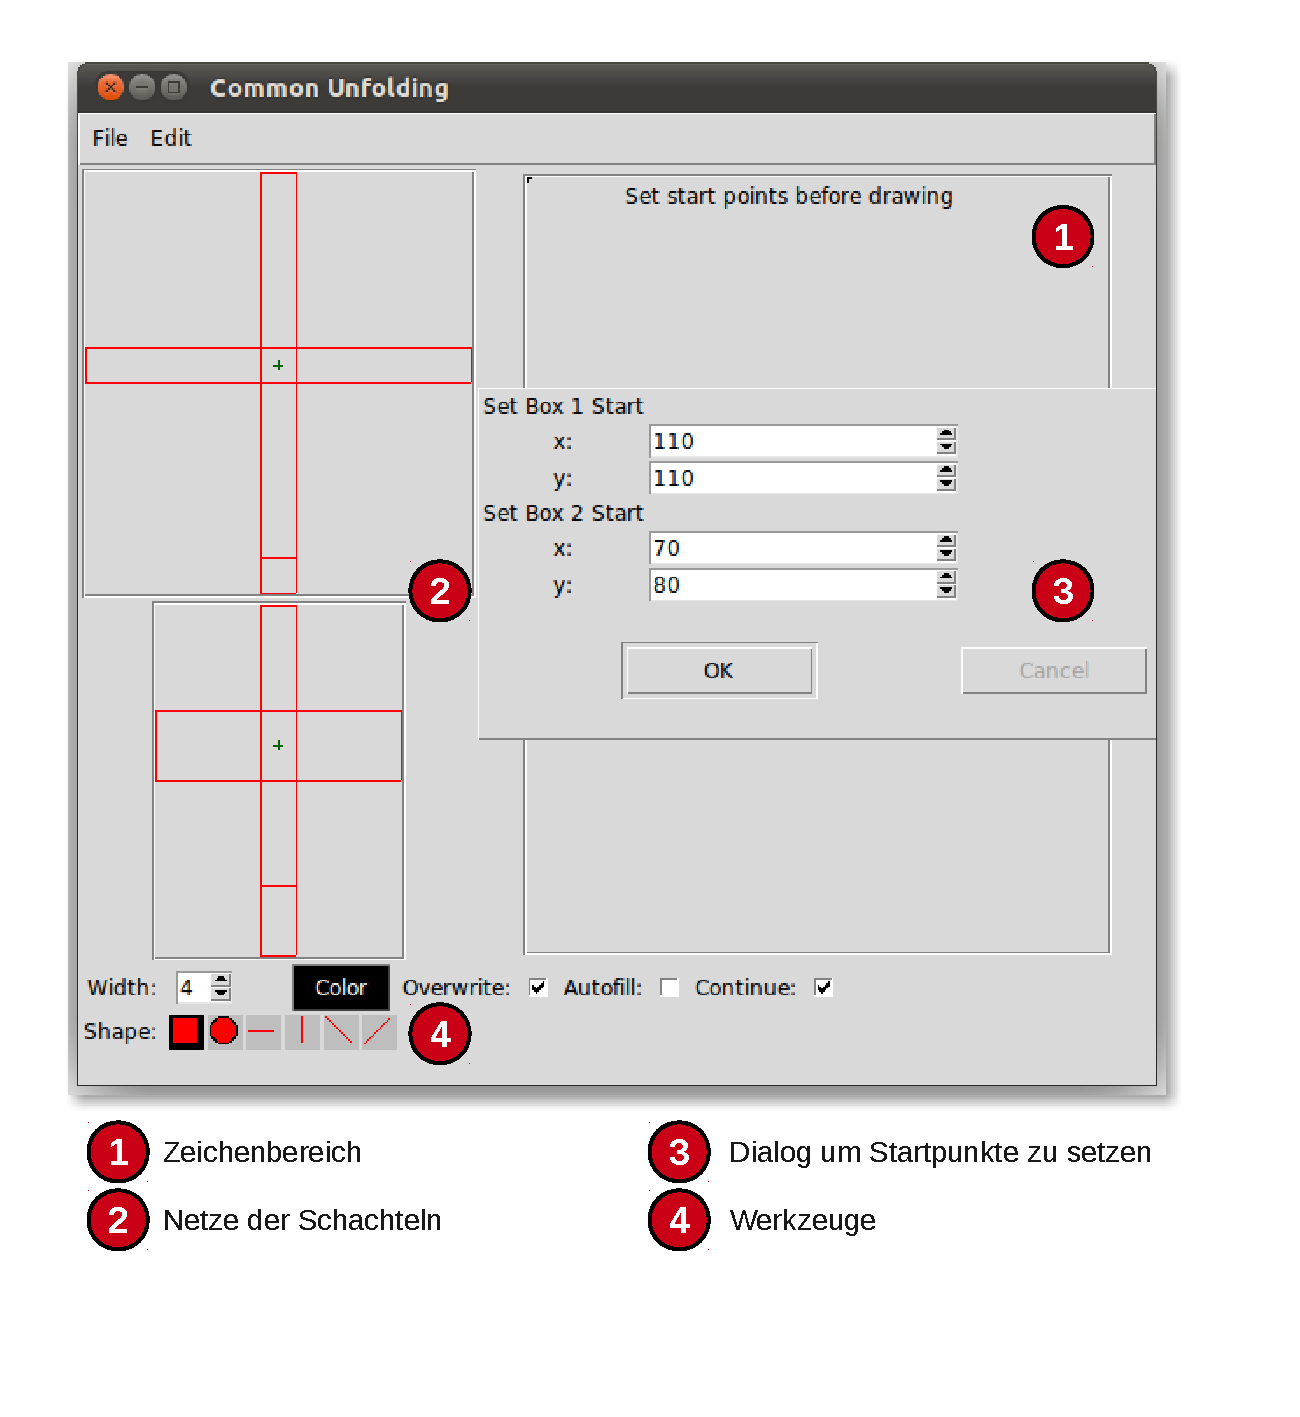
\includegraphics[scale=0.5]{03_pics/Zeichenbereich.pdf}
  \caption{Zeichenoberfläche}
  \label{fig:zeichenoberflaeche}
  \end{figure}


%%%%%%%%%%%%%%%%%%%%%%%%%%%%%%%%%%%%%%%%%%%%%%%%%%%%%%%%%%%%%%%%%%%%%%%%%%%%%%%
%%%%%%%%%%%%%%%%%%%%%%%%%%%%%%%%%%%%%%%%%%%%%%%%%%%%%%%%%%%%%%%%%%%%%%%%%%%%%%%
%%%%%%%%%%%%%%%%%%%%%%%%%%%%%%%%%%%%%%%%%%%%%%%%%%%%%%%%%%%%%%%%%%%%%%%%%%%%%%%
% LADEN, SPEICHERN, EXPORTIEREN %%%%%%%%%%%%%%%%%%%%%%%%%%%%%%%%%%%%%%%%%%%%%%%
%%%%%%%%%%%%%%%%%%%%%%%%%%%%%%%%%%%%%%%%%%%%%%%%%%%%%%%%%%%%%%%%%%%%%%%%%%%%%%%
\subsection{Datei lade, speichern, exportieren}
\label{subsec:dateioperationen}

Beschreibung wie werden Dateien geladen, gespeichert und exportiert.